% \newcommand{\hypothesis}{Advanced biomedical signal processing and machine learning algorithms can be used for efficient, high-performing analysis of sleep studies.}
% \acresetall
\chapter{Thesis introduction}\label{chap:thesis-introduction}

\begin{flushright}{\slshape 
        Quantum carburetor? Jesus, Morty, you can't just add a sci-fi word to a car word and hope it means something.} \\ \medskip
        --- Rick Sanchez\\Rick and Morty, season 2, episode 6.
\end{flushright}
\vspace{6cm}

Although sleep is essential for normal human brain development and functionality, sleep disorders are prevalent in society.
There are approximately 90 different sleep disorders currently recognized and described in the \ac{ICSD} grouped into six categories: insomnias, circadian rhythm sleep-wake disorders, central hypersomnias (\eg narcolepsy), sleep-related breathing disorders (\eg obstructive sleep apnea), parasomnias (\eg sleepwalking, \acl{RBD}), and sleep-related movement disorders (\eg \acl{PLMD} and restless legs syndrome)~\cite{AmericanAcademyofSleepMedicine2014}.
It is estimated that about 25\% of the US population present with sleep apnea-related symptoms~\cite{Young2002, Gottlieb2020} with similar prevalences in other developed countries~\cite{Tufik2010, Heinzer2015, Arnardottir2016, Fietze2019}.
The prevalence of chronic insomnia is estimated to be about 10\% of the US population~\cite{Ozminkowski2007}, and 6\% in high-income countries~\cite{Ohayon2002}---a number increasing to up to 48\% when including insomnia symptoms alone~\cite{Ohayon2002}. 
Although these numbers are high, evidence suggests that sleep disorders are severely under-diagnosed~\cite{Decker2008, Ohayon2011, Johnson2018}. 

Disrupted sleep is associated with increased risk of developing systemic hypertension, cardiovascular disease and abnormalities in the metabolism~\cite{Punjabi2008}.
Increased levels of fatigue due to disrupted nighttime sleep is also a cause of motor-vehicle accidents~\cite{Lyznicki1998}, as people with excessive daytime sleepiness have a sevenfold greater risk of being involved in an accident~\cite{Findley1988}.

Apart from the medical impacts on a personal level, sleep disorders have monumental societal impact due to their prevalence and cost of care.
A study on the burden of poor sleep in the Australian population estimated the annual economic cost at \$42.5 billion~\cite{Hillman2006}, while the combined cost of poor sleep in USA, Canada, UK, Japan and Germany is estimated to exceed \$600 billion per year~\cite{Hafner2017}. 
USA alone accounts for an estimated \$411 billion of these costs~\cite{Kiley2019}.

Currently, the gold standard of diagnosing sleep disorders is based on manual analysis of sleep patterns following the guidelines published by the \ac{AASM} and the clinical guidelines in the~\ac{ICSD}~\cite{AmericanAcademyofSleepMedicine2014}.
Sleep is recorded in sleep clinics using \ac{PSG}, which comprises several recording modalities across the body\graffito{Specific details concerning \ac{PSG} setup and recording will be described in~\cref{sec:recording-quantifying-sleep}.}.
% covers multiple modalities such as \ac{EEG} for recording brain activity, \ac{EOG} for eye movements, \ac{EMG} for chin and limb muscle activity, \ac{ECG} for heart activity, respiratory inductance plethysmopgrahy belts on the thorax and abdomen, and pulse oximetry for measuring blood oxygen content.
Patients in the sleep clinic wear and sleep with a heavy and extensive recording setup, which may have an impact on regular sleep patterns~\cite{Agnew1966, Scholle2003}.

Apart from being time consuming and cumbersome for both patients and clinical personnel, there is growing evidence\graffito{These findings on variability will be presented in~\cref{sec:challenges-scoring-sleep-studies}.} that manual analysis of sleep patterns suffer from subjectiveness resulting in high inter-scorer variabilities~\cite{Drinnan1998, Whitney1998, Danker-Hopfe2004, Norman2000, Magalang2013, Rosenberg2013, Rosenberg2014, Younes2016, Younes2018}.
In the last decades, there has been an increasing effort to come up with new solutions that can ease and standardize the way sleep data is acquired and analyzed. 
% Due to these issues, there is an increasing effort to come up with solutions that can tackle these problem areas both in terms of data acquisition and data analysis.

\begin{figure}
\begin{adjustwidth*}{}{-\marginparwidth-\marginparsep}
    \centering
    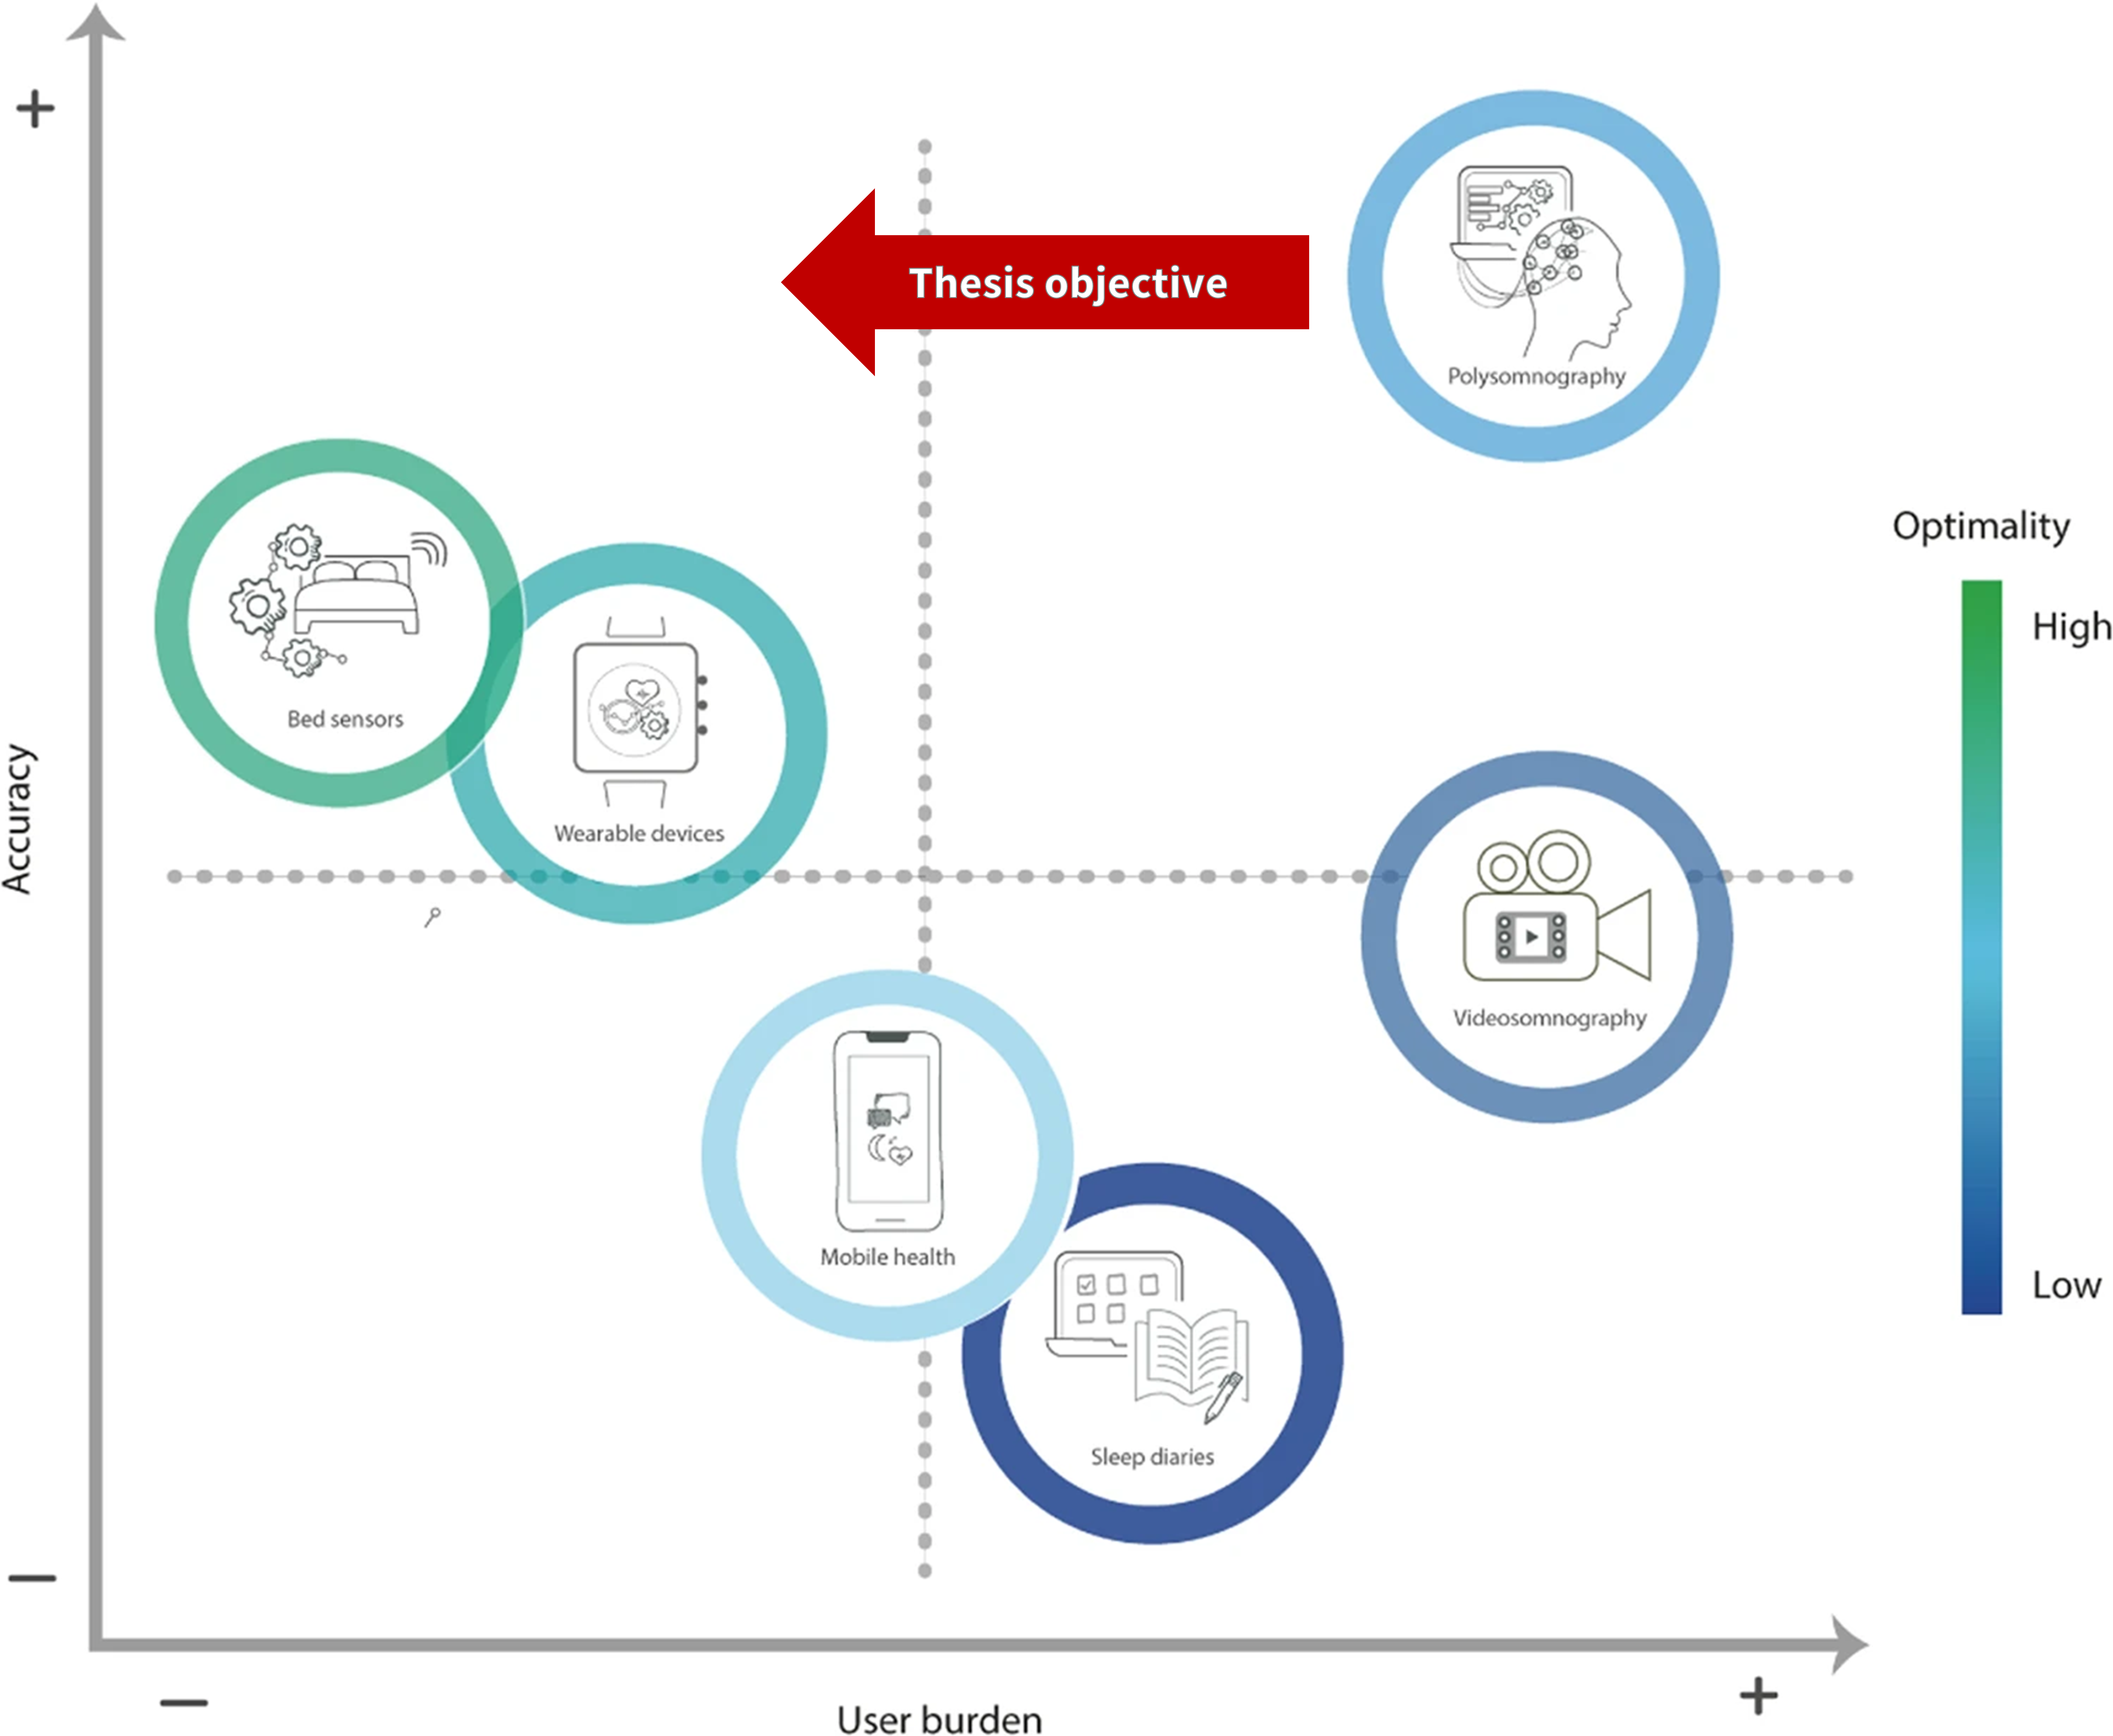
\includegraphics[width=0.95\linewidth]{figures/introduction/npjFig3_objective.png}
    \caption[Accuracy-usability trade-off in sleep analysis]{Accuracy-usability trade-off for selected methods in sleep analysis. Polysomnography is considered the gold standard in sleep medicine providing high levels of accuracy, while also being very cumbersome and time-consuming. Videosomnography provides lower levels of accuracy, while being equally cumbersome and time-consuming, although this is required for diagnosis of some sleep disorders. User-centered technologies such as health apps and sleep diaries are easier to use than the gold standard methods, but are generally not accurate in capturing sleep metrics. Wearable devices and ubiquitous technologies, such as bed and radiowave sensors, generally have the lowest impact on the user, while providing medium levels of accuracy. This thesis will focus on improving the the gold standard indicated on the figure by moving polysomnography along the red arrow to the left along the user burden axis. In this case, user burden encompasses both the burden to the patient, as well as the burden to the clinician. Adapted from~\cite{Perez-Pozuelo2020} under a Creative Commons Attributes 4.0 International License: \url{http://creativecommons.org/licenses/by/4.0/}.}
    \label{fig:introduction:figure-02}
\end{adjustwidth*}
\end{figure}

% On the acquisition side, n
Numerous commercial, industrial and academic interests are focusing on easier methods for acquiring sleep data in the form of mobile health applications and low-cost wearable/nearable devices\graffito{\emph{Nearables} include non-contact devices such as radar-based sensing, and embedded sensors such as bed sensors.} such as headbands, in-ear \ac{EEG}, or activity trackers~\cite{Perez-Pozuelo2020}.
These devices are interesting from several standpoints, but mostly due to the low user burden compared to conventional \ac{PSG}.
However, wearable devices are not yet applied in clinical practice, due to the limited validation against gold standard methods~\cite{Depner2019}.
This trade-off between usability and user burden versus accuracy is depicted graphically in~\cref{fig:introduction:figure-02} for several methods available for sleep recording and/or quantification.% of sleep.

Similarly, numerous efforts have already been made on the data analysis side to automate the sleep analysis process.
Especially the task of automatic sleep stage classification has been the subject of many research papers~\cite{Sen2014}.
With the rising presence of artificial intelligence in medicine, and deep learning in particular~\cite{LeCun2015, Yu2018, He2019}, more and more research groups are focusing on applying advanced signal processing and analysis techniques to sleep data.
Due to the vast number of different approaches regarding the number of classified sleep stages, feature extraction, classification algorithms, applied datasets, and validation approaches, direct comparison between published findings is a complex task~\cite{Ronzhina2012, Sen2014, Radha2014, Aboalayon2016, Boostani2017}.
However, high quality large-scale studies on automatic methods for sleep analysis was until very recently not dominant in the literature.
% \paragraph{Missing paragraphs}
% \begin{itemize}
%     \item Introduction to sleep science?
%     \item Introduce some papers on automating clinical sleep scoring, state of the art
%     \item (Need for objective measures since perceptions of sleep are highly subjective: 1. Hermans LWA, van Gilst MM, Regis M, et al. Modeling sleep onset misperception in insomnia. Sleep. 2020:1-10. doi:10.1093/sleep/zsaa014 \cite{Hermans2020})
%     \item New technologies for sleep analysis \cite{Perez-Pozuelo2020}
% \end{itemize}



% \begin{figure}
%     % \begin{adjustwidth*}{}{-\marginparwidth-\marginparsep}
%     \myfloatalign   
%     \subfloat[]
%     {\includegraphics[width=0.49\textwidth + 0.49\marginparwidth + 0.49\marginparsep]{figures/introduction/41746_2020_244_Fig2_HTML.pdf}} \\
%     \subfloat[]
%     {\includegraphics[width=0.49\textwidth + 0.49\marginparwidth + 0.49\marginparsep]{figures/introduction/41746_2020_244_Fig3_HTML.pdf}}
%     \caption{}
%     \label{fig:introduction:figure-01}
%     % \end{adjustwidth*}
% \end{figure}


\section{Problem statement and research hypothesis}
Analysis of sleep is based on manual scoring of \acp{PSG} recorded overnight at either a sleep clinic or at home, which are prone to subjective interpretation of scoring rules.
Correct identification and analysis of sleep patterns precedes correct diagnosis and thus subsequent treatment of sleep disorders.
\textbf{The objective of this thesis is}
\begin{quote}
    % \emph{to develop a system based on artificial intelligence, that can assist clinicians in the analysis of sleep studies.}
    \emph{\objective.}
    % \emph{to develop a system based on artificial intelligence to assist medical and technical experts in automatic analysis of sleep studies.}
\end{quote}
The aim is to ease the way \acp{PSG} are analyzed in the clinic today, but without lowering accuracy.
This is depicted graphically in~\cref{fig:introduction:figure-02} by moving the \ac{PSG} along the red arrow.
% \emph{to develop a system based on artificial intelligence to assist medical and technical experts in automatic analysis of sleep studies}.
% This is depicted graphically in~\cref{fig:introduction:figure-02} by moving the user burden of \ac{PSG} along the red arrow while maintaining high levels of accuracy.

% Taking into account the motivation, the problem statement is formalized into three separate research hypotheses:
Taking into account the motivation, the problem statement is formalized into the following \textbf{thesis hypothesis}:
\begin{quote}
    \hypothesis
\end{quote}
\begin{enumerate}[label={\footnotesize\bfseries\scshape RH~\arabic*}, ref={\bfseries\scshape RH~\arabic*}]
    \item sleep stages;\label{hypothesis:sleep-stages}%\hypothesisSleepStages;\label{hypothesis:sleep-stages}
    \item sleep events;\label{hypothesis:sleep-events} and,%\hypothesisSleepEvents;\label{hypothesis:sleep-events}
    \item sleep disorders.\label{hypothesis:sleep-disorders}%\hypothesisSleepDisorders;\label{hypothesis:sleep-events}
\end{enumerate}


% \section{Research questions and hypotheses}
% Taking into the account the motivation, the problem statement is formalized by the following \emph{thesis hypothesis}:
% \begin{quote}
%     \emph{\hypothesis}
% \end{quote}
% Based on the thesis hypothesis, the following \emph{thesis objectives} are defined:
% \begin{itemize}
%     \item to design a fully automatic sleep stage classification algorithm based on advanced machine learning techniques and validate the utility of such an algorithm in multiple databases.
%     \item to design a flexible sleep event detection algorithm that can both classify and localize sleep events in the \ac{PSG}. The algorithm should be flexible by design to allow for multiple event classes and/or signal inputs.
%     \item to design an algorithm capable of detecting sleep disorders based on a single night of \ac{PSG} recording and validate the utility of such and algorithm in multiple databases.
% \end{itemize}
% \hypothesis
% \begin{enumerate}[label={\footnotesize\bfseries\scshape RH~\arabic*}, ref={\bfseries\scshape RH~\arabic*}]
%     \item sleep stages;\label{hypothesis:sleep-stages}%\hypothesisSleepStages;\label{hypothesis:sleep-stages}
%     \item sleep micro-events; and,\label{hypothesis:sleep-events}%\hypothesisSleepEvents;\label{hypothesis:sleep-events}
%     \item sleep disorders.\label{hypothesis:sleep-disorders}%\hypothesisSleepDisorders;\label{hypothesis:sleep-disorders}.
% \end{enumerate}
% Also write something along the lines that brain activity can be represented by a mixture of states (fuzzy logic, hypnodensity)

\section{Thesis outline and scientific contributions}
\newcommand{\printpublication}[1]{\AtNextCite{\defcounter{maxnames}{99}}\fullcite{#1}}
The scientific content of this research is grouped into three research themes each with its own chapter.
% \begin{enumerate}[label={\footnotesize\bfseries\scshape Chapter~\arabic*}, ref={\bfseries\scshape Chapter~\arabic*}]
%     \item contains the preliminary introduction and motivation to this thesis, and outlines the content (about which you are now reading) and scientific contributions herein.
%     \item provides necessary clinical background for readers with little previous knowledge in somnology and sleep medicine\graffito{\emph{Somnology} is a branch of science devoted to the study of the physiology and behavioral dimensions of sleep, and the personal and population-level effects of poor sleep. \emph{Sleep medicine} is a branch of clinical medicine devoted to the diagnosis and treatment of individuals suffering from chronic sleep loss or sleep disorders.}. 
%     However, this is by now means an exhaustive treatment of the two fields.
%     \item presents three studies on \emph{automatic sleep stage classification} models, the first research theme.
%     \item presents three studies on a model developed for \emph{sleep micro-event detection}, which is the second research theme.
%     \item presents the development of a narcolepsy classification algorithm, based on outputs from one of the sleep stage classification models presented in \textbf{Chapter 3}.
%     \item integrates the findings from the three research chapters in a discussion relative to the stated research hypotheses and objectives.
%     \item concludes the thesis by summing up the main research findings.
%     \item outlines some of the future directions and research perspectives in the field of \emph{computational sleep science} related to the themes presented in this thesis.
% \end{enumerate}

\textbf{\cref{chap:thesis-introduction}} contains the preliminary introduction and motivation to this thesis, and outlines the content and scientific contributions.

\textbf{\cref{chap:clinical-background}} provides necessary clinical background for readers with little previous knowledge in somnology and sleep medicine.
%\graffito{\emph{Somnology} is a branch of science devoted to the study of the physiology and behavioral dimensions of sleep, and the personal and population-level effects of poor sleep. \emph{Sleep medicine} is a branch of clinical medicine devoted to the diagnosis and treatment of individuals suffering from chronic sleep loss or sleep disorders.}. 
% However, this is not intended to provide an exhaustive treatment of the two fields.
    
\textbf{\cref{chap:sleep-stage-classification}} presents three studies on \emph{automatic sleep stage classification}, the first research theme.

\textbf{\cref{chap:sleep-event-detection}} presents three studies on a model developed for \emph{sleep micro-event detection}, which is the second research theme.

\textbf{\cref{chap:classification-sleep-disorders}} presents the development of a narcolepsy classification algorithm, based on outputs from one of the sleep stage classification models presented in~\cref{chap:sleep-stage-classification}. This concerns the third and final research theme.

\textbf{\cref{chap:discussion}} integrates the findings of this dissertation in a discussion relative to the stated research hypotheses and objectives.

\textbf{\cref{chap:conclusion}} concludes the thesis by summing up the main research findings.

\textbf{\cref{chap:future-work}} outlines some of the future directions and research perspectives in the field of \emph{computational sleep science}.

\bigskip

The following first-author publications have been published, accepted or submitted during my PhD studies and form the scientific basis of this thesis.\footnote{\(^{\ast}\) indicates shared first authorship.} Preprints and/or published versions of these are supplied in the appendix.
    
\begin{refsection}[ownpubs]
    \small
    
    \paragraph{Journal papers}
    \begin{itemize}[label=--]
        \item \printpublication{Stephansen2018}
        \item \printpublication{Olesen2020AutomaticSetting}
        \item \printpublication{Olesen2020MSED}
    \end{itemize}
    
    \paragraph{Conference papers}
    \begin{itemize}[label=--]
        \item \printpublication{Olesen2018c}
        \item \printpublication{Olesen2019}
        \item \printpublication{Olesen2020DeepDetection}
    \end{itemize}
\end{refsection}

\noindent Furthermore, I have (co-)authored the following publications during my PhD.%, that although relevant, do not form basis of this thesis.

\begin{refsection}[ownpubs]
    \small
    \paragraph{Journal papers}
        \begin{itemize}[label=--]
            \item \printpublication{Olesen2018}
            \item \printpublication{Cesari2018}
            \item \printpublication{Brink-Kjaer2020}
            \item \printpublication{Carvelli2020}
            \item \printpublication{Ambati2020}
        \end{itemize}
        
    \paragraph{Conference papers}
    \begin{itemize}[label=--]
        \item \printpublication{Klok2018}
    \end{itemize}
    
    \paragraph{Abstracts}
    \begin{itemize}[label=--]
        \item \printpublication{Brink-Kjaer2018}
        \item \printpublication{Carvelli2018}
        \item \printpublication{Jacobsen2018}
        \item \printpublication{Olesen2018a}
        \item \printpublication{Olesen2019a}
        \item \printpublication{Thybo2020}
    \end{itemize}
    
\end{refsection}


\noindent Finally, I have also written a popular science article about my research titled \emph{Intelligente algoritmer på søvnklinikken} (Intelligent algorithms in the sleep clinic) for the Danish industry magazine \emph{Medicoteknik}.